\documentclass[UTF-8, a4paper, 12pt]{ctexart}

\usepackage[left=1in,right=1in,top=1.00in,bottom=1.00in]{geometry}
\usepackage[colorlinks,linkcolor=blue,anchorcolor=blue,citecolor=green,CJKbookmarks=True]{hyperref}
%\usepackage{CJK,CJKnumb}        % 在 mac 下将此行注释掉
%\usepackage{indentfirst}        % 首行缩进宏包
%\usepackage{latexsym,bm}        % 处理数学公式中和黑斜体的宏包
\usepackage{amsmath,amssymb}     % AMSLaTeX宏包 用来排出更加漂亮的公式
\usepackage{graphicx}
\usepackage{cases}
\usepackage{pifont}
\usepackage{txfonts}
\usepackage{subfigure}
\usepackage{pdfpages}
\usepackage{listings}
\usepackage{xcolor}
\usepackage[subfigure]{tocloft}     % 模板中用了subfigure,不加此选项会产生冲突
\usepackage{inconsolata}
\CTEXsetup[format={\Large\bfseries}]{section}
\zihao{-4}\linespread{1.5}\selectfont
\renewcommand{\theequation}{\arabic{section}-\arabic{equation}}
\renewcommand{\thefigure}{\arabic{section}-\arabic{figure}}
%\renewcommand{\thefigure}{\thechapter-\arabic{figure}}
\renewcommand{\cftsecleader}{\cftdotfill{\cftdotsep}}
\renewcommand\contentsname{{\qquad\qquad\qquad\qquad\qquad\qquad 目\quad 录}}
\newcommand{\song}{\CJKfamily{song}}    % 宋体   (Windows自带simsun.ttf)


%=====================
%用来设置附录中代码的样式
% 头文件
\usepackage{listings} 
\usepackage{fontspec}
\setmonofont{Consolas}
%\begin{lstlisting}[
%	language = matlab, numbers=left, 
%	numberstyle=\tiny,keywordstyle=\color{blue!70},
%	commentstyle=\color{red!50!green!50!blue!50},frame=shadowbox,
%	rulesepcolor=\color{red!20!green!20!blue!20},
%	basicstyle=\ttfamily,
%	]
%	
%\end{lstlisting}
%=====================




\title{\bfseries \Huge  }
\author{}
\date{}





\begin{document}
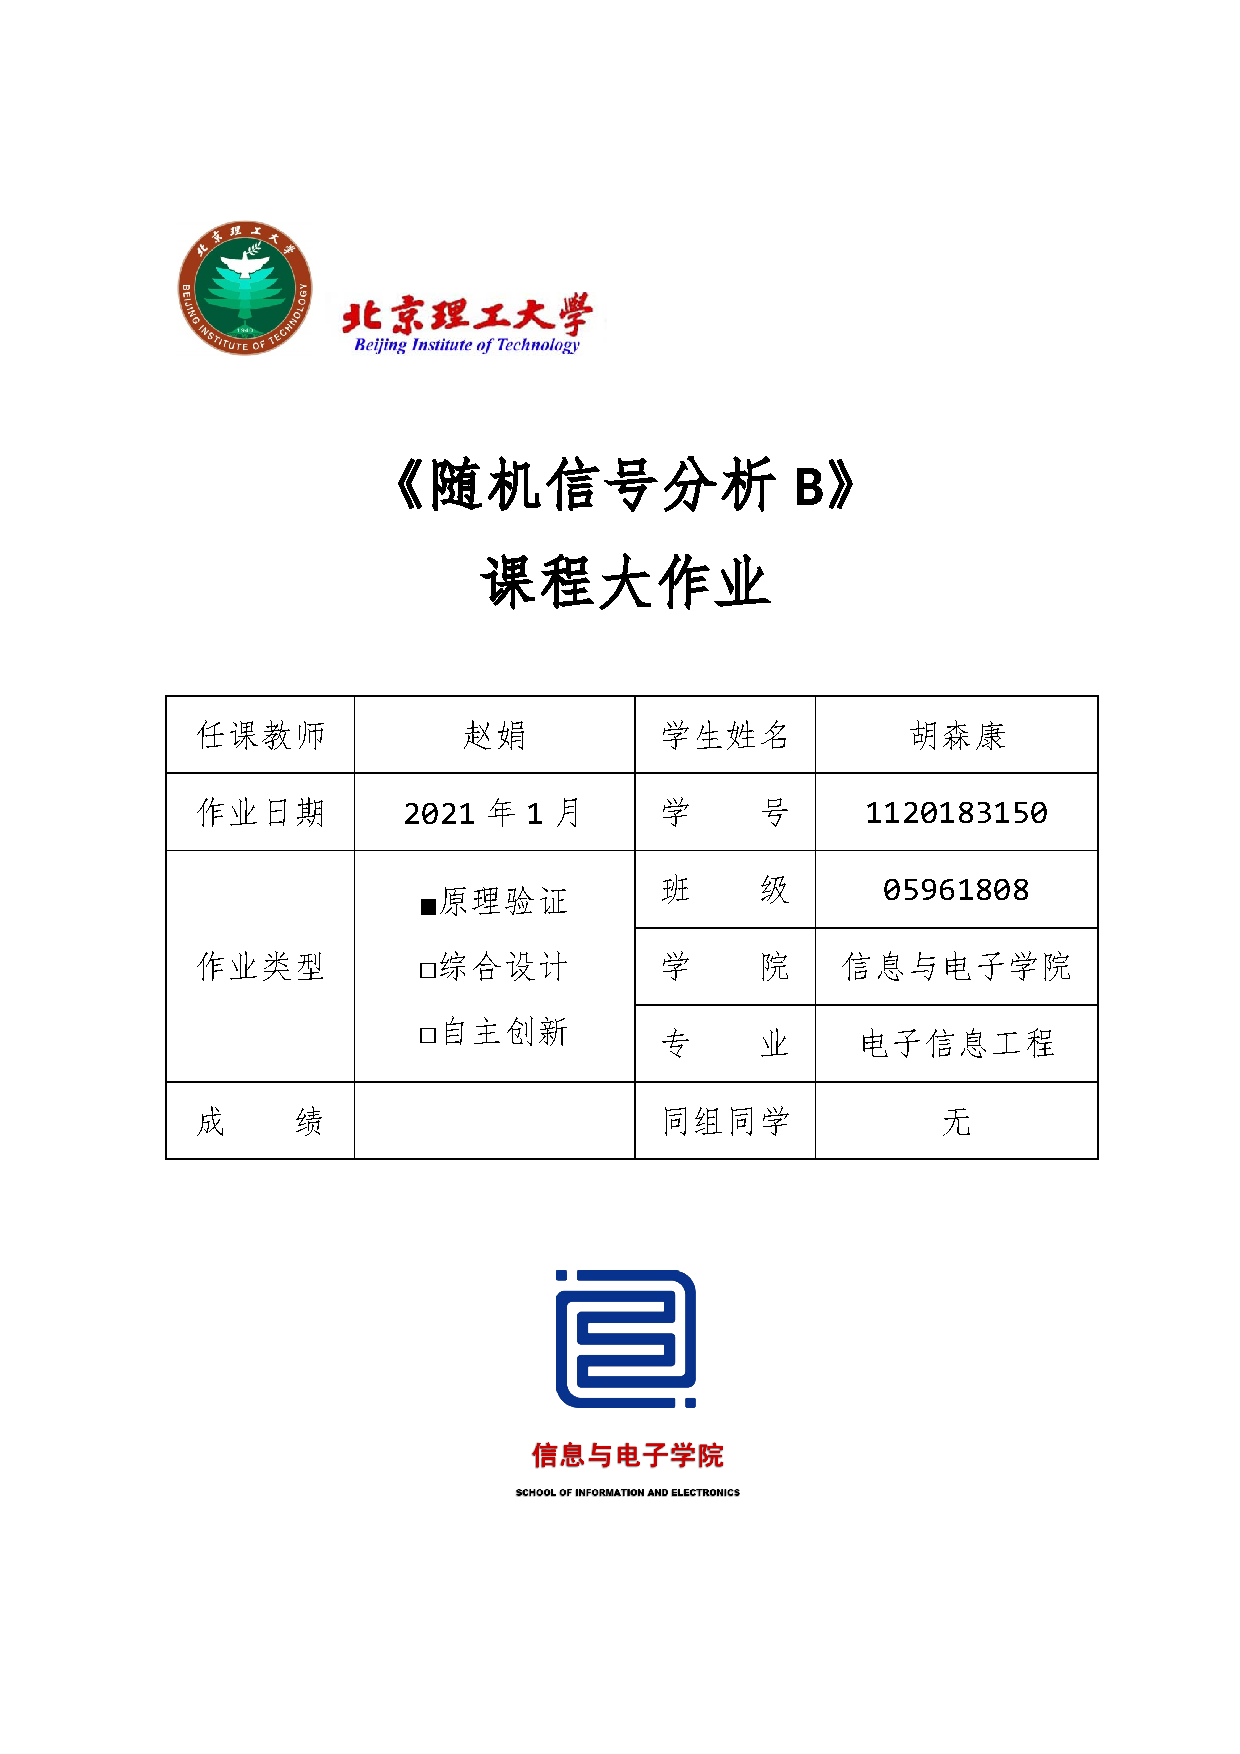
\includepdf[pages={1}]{coverpage.pdf} %% 插入pdf

%\maketitle

%\thispagestyle{empty}
%\newpage
%\thispagestyle{empty}


\tableofcontents

\newpage

\section{平稳随机过程的谱分析题目一}

产生不同带宽的宽平稳和宽遍历随机序列的若干样本,
    考察样本序列时域起伏程度与带宽的定性关系,画出序列的自
    相关函数和功率谱密度;

\subsection{研究思路}
\begin{enumerate}
    \item 利用MATLAB产生高斯随机序列
    \item 利用MATLAB设计带通滤波器
    \item 改变带通滤波器的带宽
    \item 将高斯随机序列通过此带通滤波器
    \item 定性地观察带通滤波器输出的随机序列的起伏程度
    \item 画出序列的自相关函数和功率谱密度
\end{enumerate}
\subsection{研究过程}

1. 利用MATLAB产生高斯随机序列
\begin{lstlisting}[
	language = matlab, numbers=left, 
	numberstyle=\tiny,keywordstyle=\color{blue!70},
	commentstyle=\color{red!50!green!50!blue!50},frame=shadowbox,
	rulesepcolor=\color{red!20!green!20!blue!20},
	basicstyle=\ttfamily,
	]
fs=10000;
x=randn(1000,1);
\end{lstlisting}

2. 设计带通滤波器
\begin{lstlisting}[
	language = matlab, numbers=left, 
	numberstyle=\tiny,keywordstyle=\color{blue!70},
	commentstyle=\color{red!50!green!50!blue!50},frame=shadowbox,
	rulesepcolor=\color{red!20!green!20!blue!20},
	basicstyle=\ttfamily,
	]
[b,a]=ellip(10,0.5,50,[2000,4000]*2/fs);
[H,w]=freqz(b,a);
\end{lstlisting}


3. 将高斯随机序列通过此带通滤波器,并观察图形
\begin{lstlisting}[
	language = matlab, numbers=left, 
	numberstyle=\tiny,keywordstyle=\color{blue!70},
	commentstyle=\color{red!50!green!50!blue!50},frame=shadowbox,
	rulesepcolor=\color{red!20!green!20!blue!20},
	basicstyle=\ttfamily,
	]
y=filter(b,a,x);
plot(y);grid on;
\end{lstlisting}

4. 画出序列的自相关函数和功率谱密度
\begin{lstlisting}[
	language = matlab, numbers=left, 
	numberstyle=\tiny,keywordstyle=\color{blue!70},
	commentstyle=\color{red!50!green!50!blue!50},frame=shadowbox,
	rulesepcolor=\color{red!20!green!20!blue!20},
	basicstyle=\ttfamily,
	]
y_corr=xcorr(y,'unbiased');
plot(y_corr);grid on; % 画出序列的自相关函数
py=periodogram(y);
plot(py);             % 画出序列的功率谱密度
grid on;
\end{lstlisting}

\subsection{研究结果}
1. 设置带通滤波器的带通频率为$1kHz\sim 4kHz$,所得到的带通滤波器的频谱、信号的时域波形
、自相关函数和功率谱如下:
\begin{figure}[htbp]
    \centering
    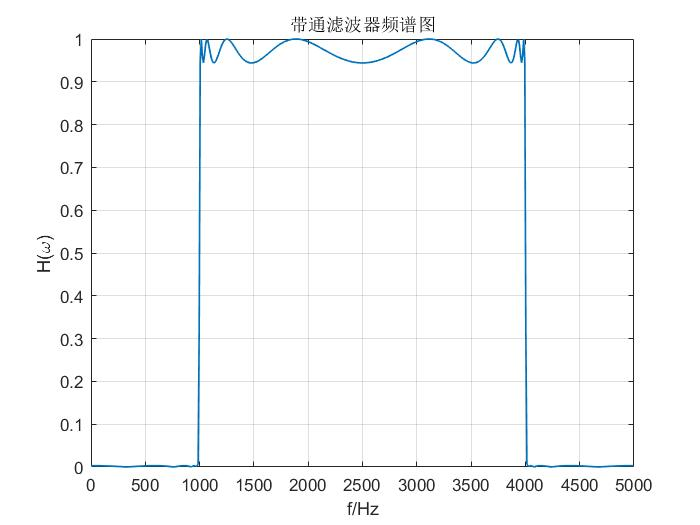
\includegraphics[width=9.5cm]{figs/f1_1.jpg}
    \caption{带通滤波器频谱 ($1kHz\sim 4kHz$)}
\end{figure}
\begin{figure}[htbp]
    \centering
    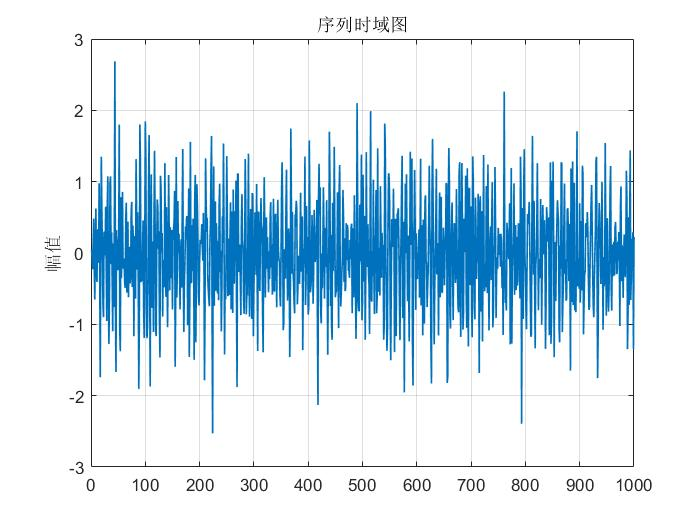
\includegraphics[width=9.5cm]{figs/f1-2.jpg}
    \caption{信号时域波形($1kHz\sim 4kHz$)}
    \label{f12}
\end{figure}
\begin{figure}[htbp]
    \centering
    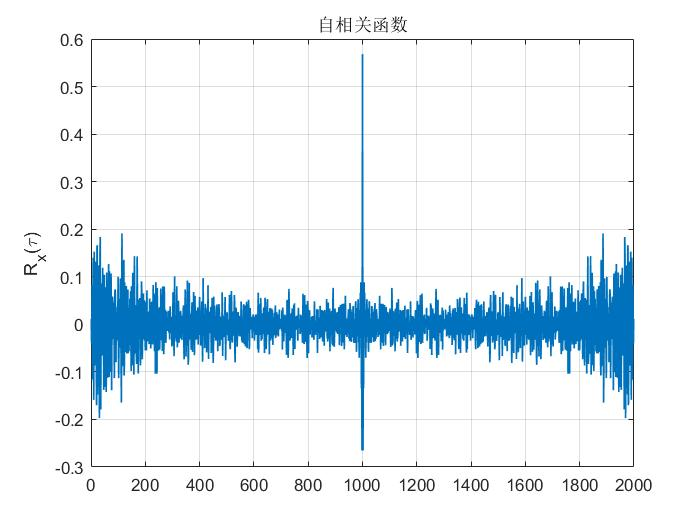
\includegraphics[width=10cm]{figs/f1_3.jpg}
    \caption{信号的自相关函数($1kHz\sim 4kHz$)}
\end{figure}
\begin{figure}[htbp]
    \centering
    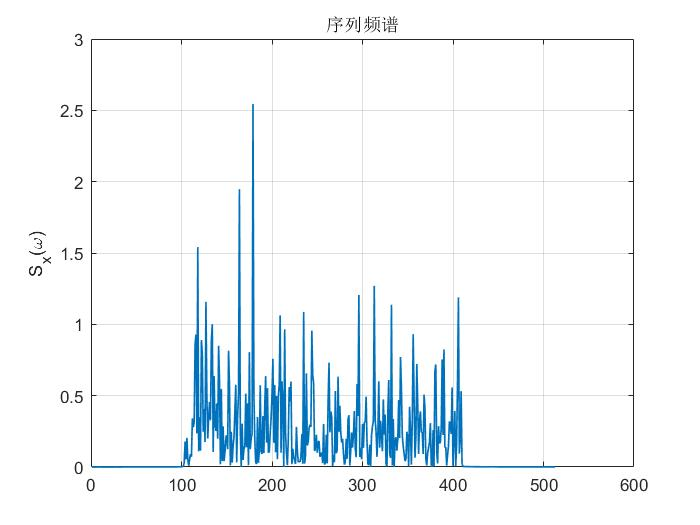
\includegraphics[width=10cm]{figs/f1_4.jpg}
    \caption{信号的功率谱密度($1kHz\sim 4kHz$)}
\end{figure}

\newpage
2. 设置带通滤波器的带通频率为$2kHz\sim 4kHz$,所得到的带通滤波器的频谱、信号的时域波形
、自相关函数和功率谱如下:
\begin{figure}[htbp]
    \centering
    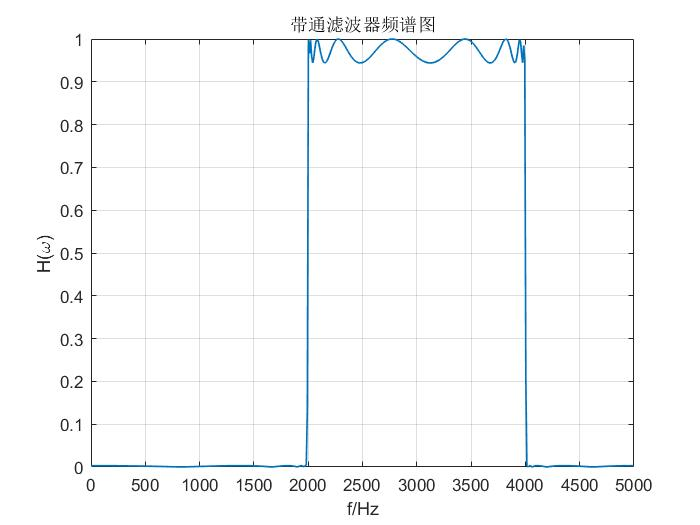
\includegraphics[width=10cm]{figs/f21.jpg}
    \caption{带通滤波器频谱($2kHz\sim 4kHz$)}
\end{figure}
\begin{figure}[htbp]
    \centering
    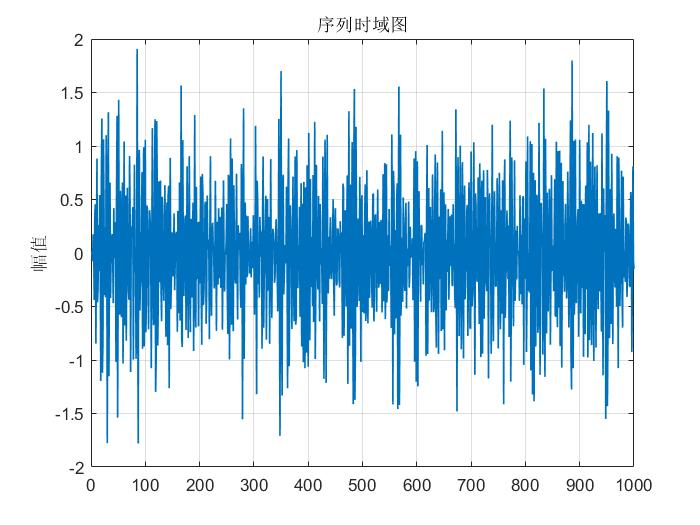
\includegraphics[width=10cm]{figs/f22.jpg}
    \caption{信号时域波形($2kHz\sim 4kHz$)}
    \label{f22}
\end{figure}
\begin{figure}[htbp]
    \centering
    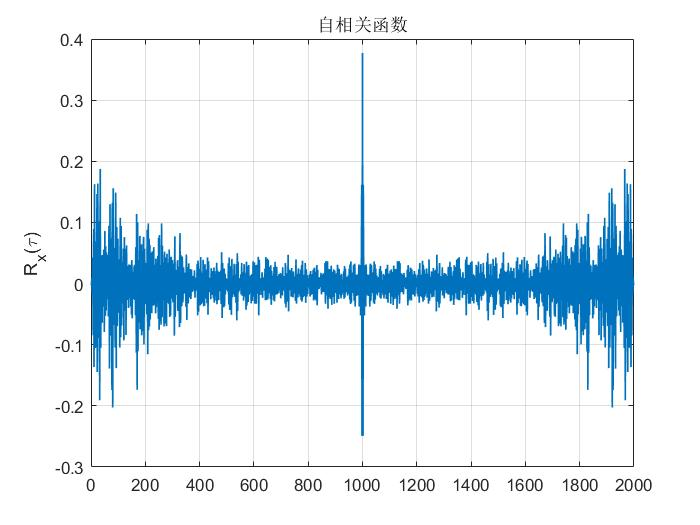
\includegraphics[width=10cm]{figs/f23.jpg}
    \caption{信号的自相关函数($2kHz\sim 4kHz$)}
\end{figure}
\begin{figure}[htbp]
    \centering
    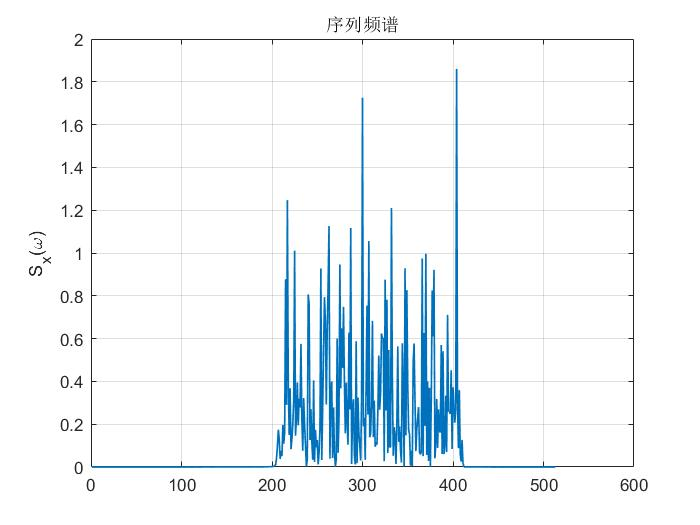
\includegraphics[width=10cm]{figs/f2_4.jpg}
    \caption{信号的功率谱密度($2kHz\sim 4kHz$)}
\end{figure}
\newpage
3. 设置带通滤波器的带通频率为$3kHz\sim 4kHz$,所得到的带通滤波器的频谱、信号的时域波形
、自相关函数和功率谱如下:
\begin{figure}[htbp]
    \centering
    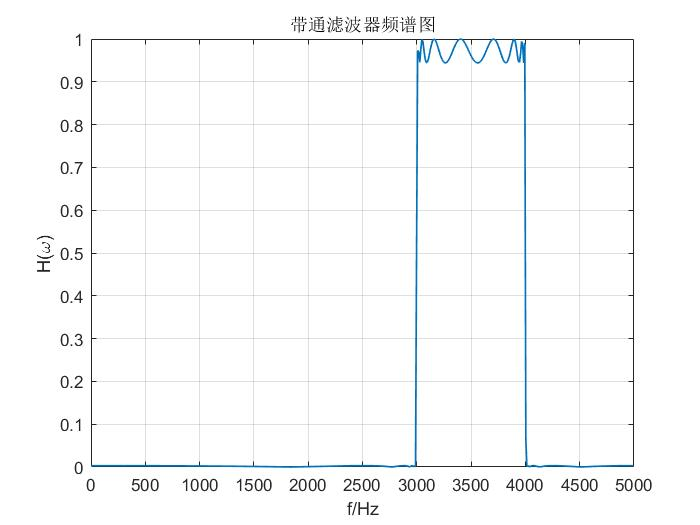
\includegraphics[width=10cm]{figs/f31.jpg}
    \caption{带通滤波器频谱($3kHz\sim 4kHz$)}
\end{figure}
\begin{figure}[htbp]
    \centering
    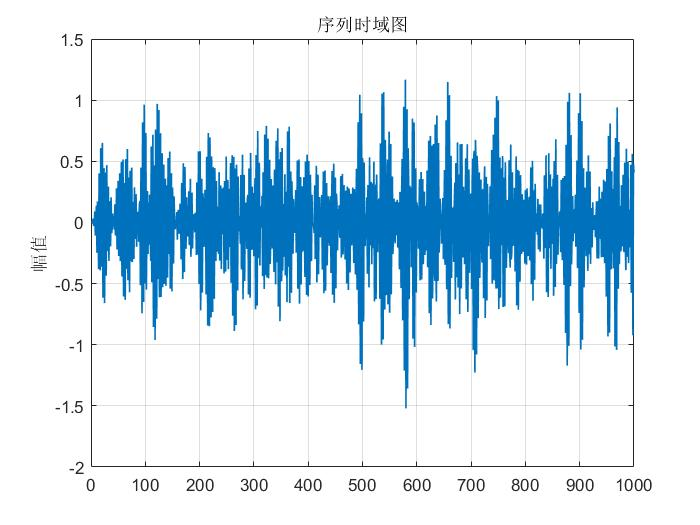
\includegraphics[width=10cm]{figs/f32.jpg}
    \caption{信号时域波形($3kHz\sim 4kHz$)}
    \label{f32}
\end{figure}
\begin{figure}[htbp]
    \centering
    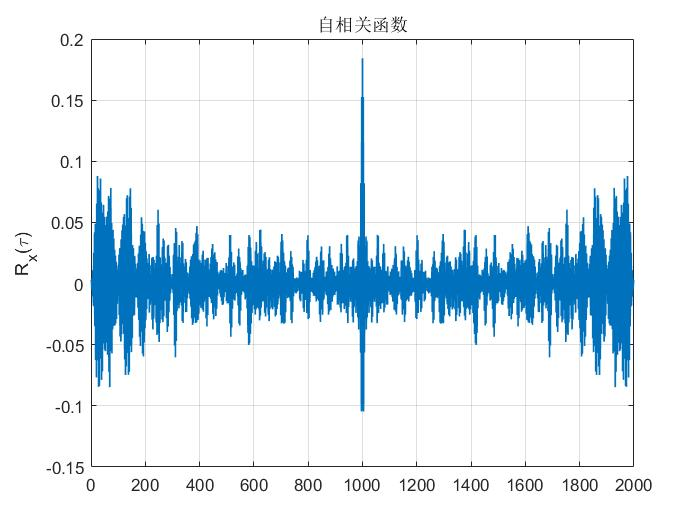
\includegraphics[width=10cm]{figs/f33.jpg}
    \caption{信号的自相关函数($3kHz\sim 4kHz$)}
\end{figure}
\begin{figure}[htbp]
    \centering
    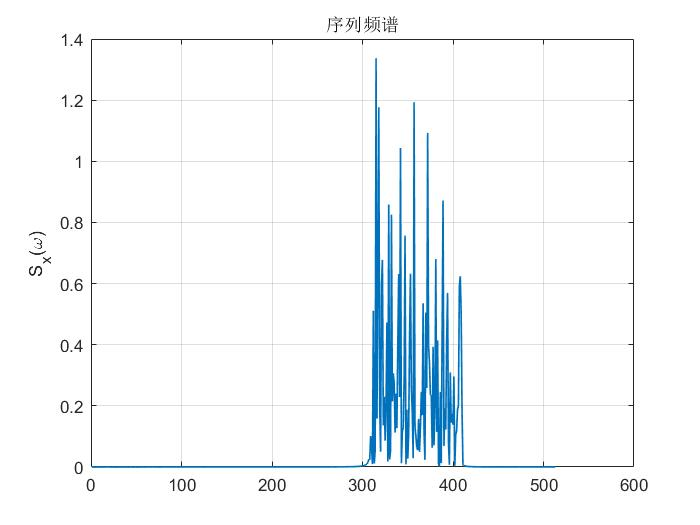
\includegraphics[width=10cm]{figs/f34.jpg}
    \caption{信号的功率谱密度($3kHz\sim 4kHz$)}
\end{figure}
\newpage
4. 设置带通滤波器的带通频率为$3.5kHz\sim 4kHz$,所得到的带通滤波器的频谱、信号的时域波形
、自相关函数和功率谱如下:
\begin{figure}[htbp]
    \centering
    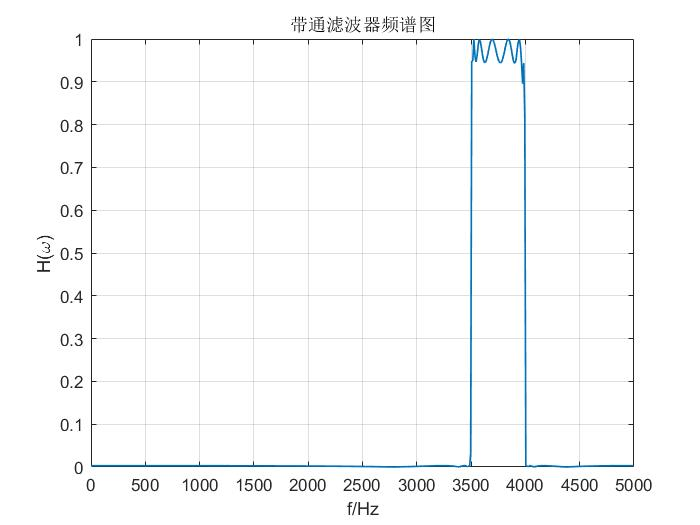
\includegraphics[width=10cm]{figs/f41.jpg}
    \caption{带通滤波器频谱($3.5kHz\sim 4kHz$)}
\end{figure}
\begin{figure}[htbp]
    \centering
    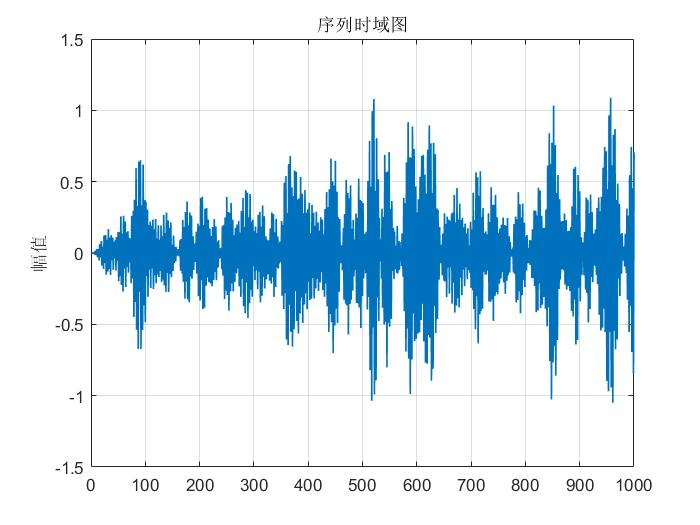
\includegraphics[width=10cm]{figs/f42.jpg}
    \caption{信号时域波形($3.5kHz\sim 4kHz$)}
    \label{f42}
\end{figure}
\begin{figure}[htbp]
    \centering
    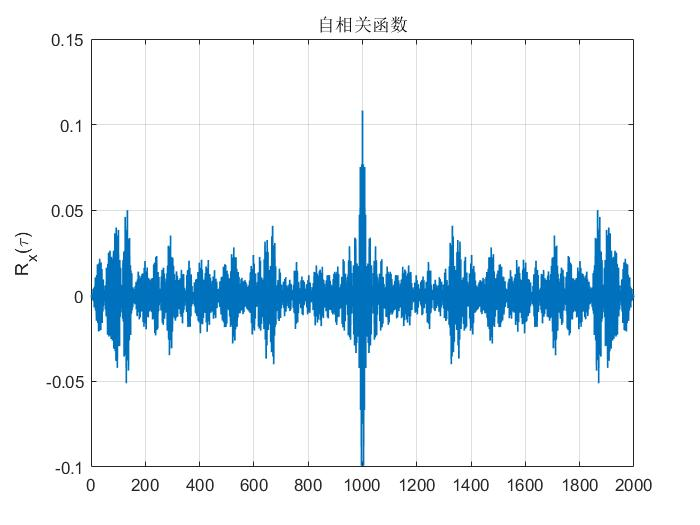
\includegraphics[width=10cm]{figs/f43.jpg}
    \caption{信号的自相关函数($3.5kHz\sim 4kHz$)}
\end{figure}
\begin{figure}[htbp]
    \centering
    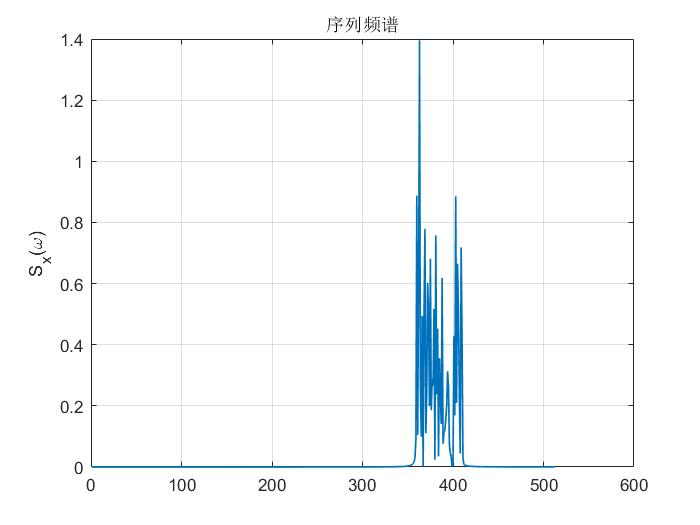
\includegraphics[width=10cm]{figs/f44.jpg}
    \caption{信号的功率谱密度($3.5kHz\sim 4kHz$)}
\end{figure}\newpage

\subsection{结果分析}
比较图(\ref{f12})、(\ref{f22})、
(\ref{f32})和(\ref{f42})的起伏程度,图像对比如下:
\begin{figure}[htbp]
    \centering
    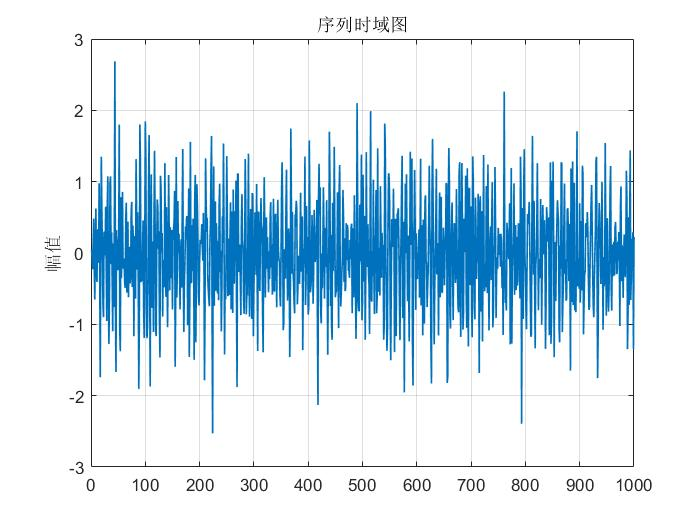
\includegraphics[width=7.5cm]{figs/f1-2.jpg}
    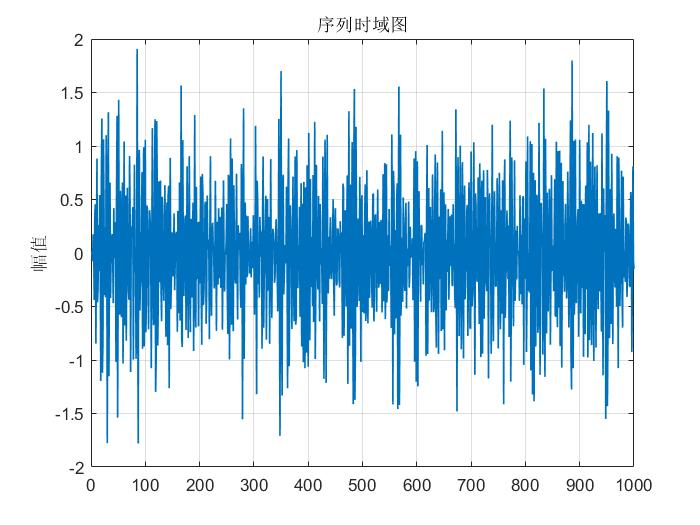
\includegraphics[width=7.5cm]{figs/f22.jpg}
    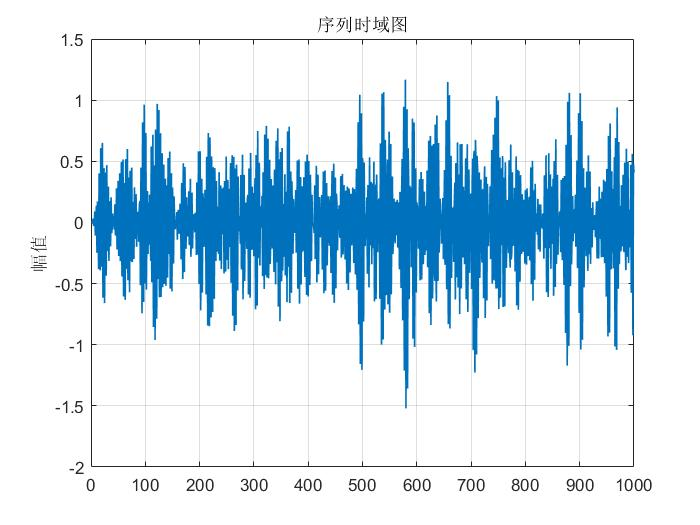
\includegraphics[width=7.5cm]{figs/f32.jpg}
    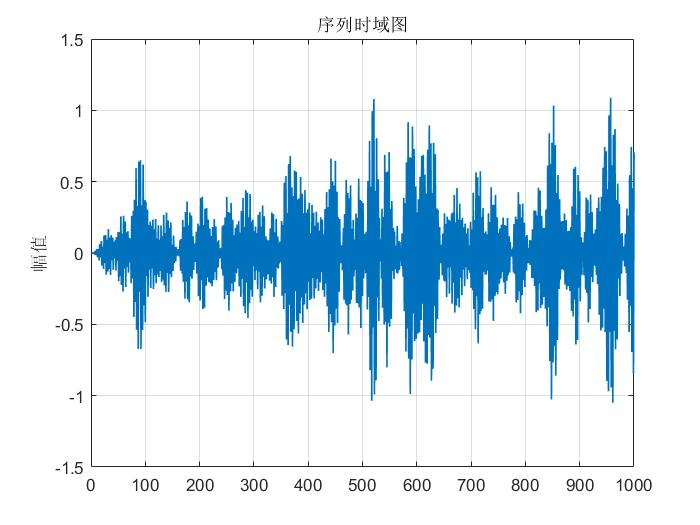
\includegraphics[width=7.5cm]{figs/f42.jpg}
\end{figure}

可定性地得出结论:{\bfseries 宽平稳和宽遍历随机序列的带宽越窄,其起伏程度越小。
}

通过MATLAB得到序列的带宽($\Delta B$)和序列的方差($\sigma^2$)之间的函数关系,
图像如图(\ref{f5})所示:
\begin{figure}[htbp]
    \centering
    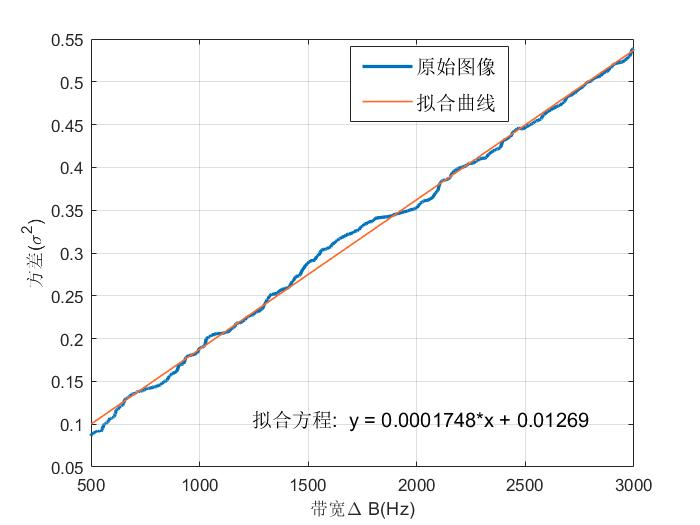
\includegraphics[width=15cm]{figs/f5.jpg}
    \caption{信号带宽和方差的关系曲线}
    \label{f5}
\end{figure}

并通过拟合得到方差和带宽具有线性关系,且关系式为$\sigma^2=0.0001748\cdot\Delta B+0.01269$
\newpage
\section{平稳随机过程的谱分析题目二}

某数字系统输出为两个不同频率正弦序列与零均值白噪
    声序列的和,推导该输出的理论功率谱密度,按功率谱密度的两
    种定义设计一种功率谱密度估计方法,画出对应于不同频率组合
    的功率谱图,解释观察到的现象。

\subsection{理论公式推导}
设输出的序列为:
\begin{equation}
    x(n)=A\cos(\omega_1n+\Phi )+B\cos(\omega_2n+\Theta )+N(n)
\end{equation}
其中$\Phi\sim U[0,2\pi]$,$\Theta\sim U[0,2\pi]$。

其自相关函数为:
\begin{equation}
    \begin{array}{ll}
     R_x(n,n+m)&=E[x(n)\cdot x(n+m)]    \\
                &=\frac{1}{2}A^2\cos\omega_1m
                +\frac{1}{2}B^2\cos\omega_1m+\frac{n_0}{2}\delta(m)\\
                &=R_x(m)
    \end{array}
\end{equation}

根据维纳-辛钦定理:
\begin{equation}
        S_x(\omega)=\sum_{m=-\infty}^{\infty}R_x(m)e^{-j\omega m}
\end{equation}

可知功率谱密度为:
\begin{equation}
    \begin{array}{rcl}
        S_x(\omega)&=&\sum_{m=-\infty}^{\infty}R_x(m)e^{-j\omega m}\\
        &=&\frac{1}{2}\pi A^2\sum^{\infty}_{m=-\infty}(\delta(\omega-\omega_1-2\pi m)+\delta(\omega+\omega_1-2\pi m))\\
        &&+\frac{1}{2}\pi B^2\sum^{\infty}_{m=-\infty}(\delta(\omega-\omega_2-2\pi m)+\delta(\omega+\omega_2-2\pi m))+\frac{n_0}{2}
    \end{array}
\end{equation}
\subsection{直接法求功率谱密度}

直接法先计算N个数据的Fourier 变换(即频谱)。
\begin{equation}
    X_N(\omega)=\sum_{n=0}^{N-1}x(n)e^{-j\omega n}
\end{equation}
然后取频谱和其共轭的乘积,得到功率谱:
\begin{equation}
    S_x(\omega)=\frac{1}{N}\left\lvert X_N(\omega)\right\rvert ^2=\frac{1}{N}\left\lvert \sum_{n=0}^{N-1}x(n)e^{-j\omega n}\right\rvert^2 
\end{equation}
\subsubsection{研究过程}
1. 利用MATLAB产生两个正弦随机序列,并产生一个加性高斯白噪声
\begin{lstlisting}[
	language = matlab, numbers=left, 
	numberstyle=\tiny,keywordstyle=\color{blue!70},
	commentstyle=\color{red!50!green!50!blue!50},frame=shadowbox,
	rulesepcolor=\color{red!20!green!20!blue!20},
	basicstyle=\ttfamily,
	]
s1 = 20*cos(2*pi*300*t+2*pi*rand); % 信号1,幅值20,频率300Hz
s2 = 10*cos(2*pi*100*t+2*pi*rand); % 信号2,幅值10,频率100Hz
ran1 = randn(1,L);                 % 产生高斯白噪声
s = s1+s2+ran1;
\end{lstlisting}

2. 通过直接功率谱估计的方法得到信号的功率谱
\begin{lstlisting}[
	language = matlab, numbers=left, 
	numberstyle=\tiny,keywordstyle=\color{blue!70},
	commentstyle=\color{red!50!green!50!blue!50},frame=shadowbox,
	rulesepcolor=\color{red!20!green!20!blue!20},
	basicstyle=\ttfamily,
	]
for i = 1:N
    [p,f1] = periodogram(s,[],nFFT,fs);
    sum1 = sum1+p;  
end
\end{lstlisting}

3. 最后得到所估计的功率谱密度的图像
\begin{lstlisting}[
	language = matlab, numbers=left, 
	numberstyle=\tiny,keywordstyle=\color{blue!70},
	commentstyle=\color{red!50!green!50!blue!50},frame=shadowbox,
	rulesepcolor=\color{red!20!green!20!blue!20},
	basicstyle=\ttfamily,
	]
plot(f1,10*log10(p),'linewidth',1);grid on;
title('直接法估计功率谱');
ylabel('S_x(\omega) (dB)');
xlabel('Frequency (Hz)');
\end{lstlisting}
\newpage
\subsubsection{研究结果}
1. 当$f_1=50Hz$,$ f_2=300Hz$,得到的结果如下图(\ref{p1})所示,
其中$S_x(\omega)$用$dB$表示。
\begin{figure}[htbp]
    \centering
    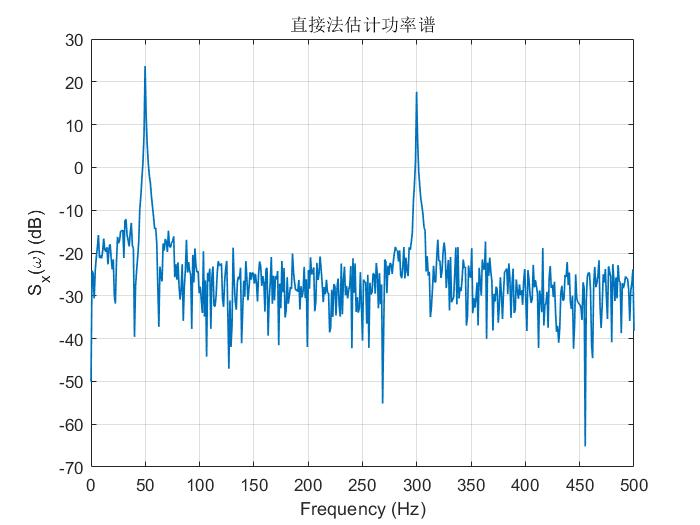
\includegraphics[width=10cm]{figs/f61.jpg}
    \caption{当$f_1=50Hz$,$f_2=300Hz$时的功率谱密度$S_x(\omega)$}
    \label{p1}
\end{figure}

2. 当$f_1=100Hz$,$ f_2=300Hz$,得到的结果如下图(\ref{p2})所示,
其中$S_x(\omega)$用$dB$表示。
\begin{figure}[htbp]
    \centering
    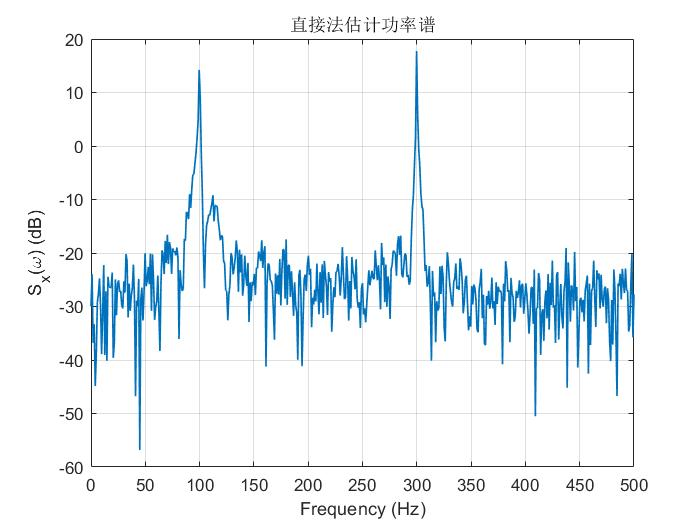
\includegraphics[width=10cm]{figs/f62.jpg}
    \caption{当$f_1=100Hz$,$f_2=300Hz$时的功率谱密度$S_x(\omega)$}
    \label{p2}
\end{figure}

3. 当$f_1=150Hz$,$ f_2=250Hz$,得到的结果如下图(\ref{p3})所示,
其中$S_x(\omega)$用$dB$表示。
\begin{figure}[htbp]
    \centering
    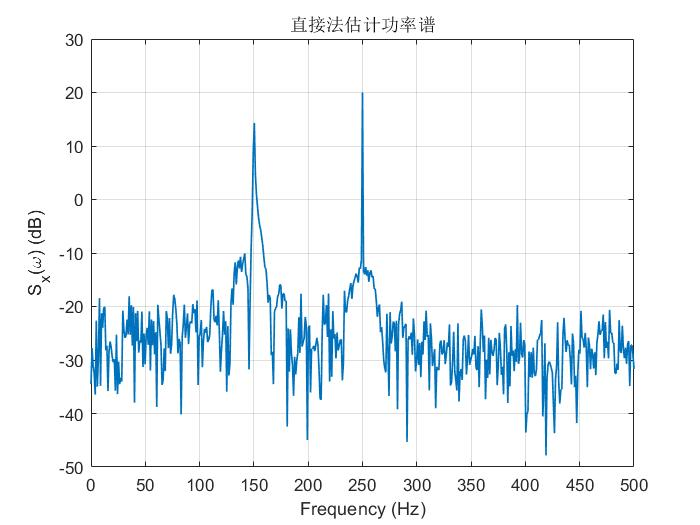
\includegraphics[width=10cm]{figs/f63.jpg}
    \caption{当$f_1=150Hz$,$f_2=250Hz$时的功率谱密度$S_x(\omega)$}
    \label{p3}
\end{figure}
\subsubsection{结果分析}
当改变正弦序列的频率组合,其功率谱密度上对应频率出现一个脉冲,
这与理论推到而来的公式是一致的。

\subsection{间接法求功率谱密度}
间接法是根据$N$个样本数据估计$x(n)$的样本自相关函数。
\begin{equation}
    R_x(m)=\frac{1}{N}\sum^{N-1}_{n=0}x^\ast(n)x(n+m), n=0,1,\cdots,M
\end{equation}
其中$1\ll M< N $,且$R_x(-m)=R_x^\ast(m)$。此后,根据维纳-辛钦定理
得出随机序列的功率谱密度。
\begin{equation}
    S_x(\omega)=\sum_{m=-\infty}^{\infty}R_x(m)e^{-j\omega m}
\end{equation}

\subsubsection{研究过程}
1. 利用MATLAB产生两个正弦随机序列,并产生一个加性高斯白噪声
\begin{lstlisting}[
	language = matlab, numbers=left, 
	numberstyle=\tiny,keywordstyle=\color{blue!70},
	commentstyle=\color{red!50!green!50!blue!50},frame=shadowbox,
	rulesepcolor=\color{red!20!green!20!blue!20},
	basicstyle=\ttfamily,
	]
s1 = 20*cos(2*pi*300*t+2*pi*rand); % 信号1,幅值20,频率300Hz
s2 = 10*cos(2*pi*100*t+2*pi*rand); % 信号2,幅值10,频率100Hz
ran1 = randn(1,L);                 % 产生高斯白噪声
s = s1+s2+ran1;
\end{lstlisting}

2. 通过直接功率谱估计的方法得到信号的功率谱
\begin{lstlisting}[
	language = matlab, numbers=left, 
	numberstyle=\tiny,keywordstyle=\color{blue!70},
	commentstyle=\color{red!50!green!50!blue!50},frame=shadowbox,
	rulesepcolor=\color{red!20!green!20!blue!20},
	basicstyle=\ttfamily,
	]
for i = 1:N
    Rm = xcorr(s,'biased');         %估计自相关函数
    p = abs(fft(Rm,nFFT))/fs;       %求得估计的功率谱
    sum2 = sum2 + p;
end
\end{lstlisting}

3. 最后得到所估计的功率谱密度的图像
\begin{lstlisting}[
	language = matlab, numbers=left, 
	numberstyle=\tiny,keywordstyle=\color{blue!70},
	commentstyle=\color{red!50!green!50!blue!50},frame=shadowbox,
	rulesepcolor=\color{red!20!green!20!blue!20},
	basicstyle=\ttfamily,
	]
plot(f2,10*log10(2*p(1:nFFT/2)),'linewidth',1);grid on;
title('间接法估计功率谱');
ylabel('S_x(\omega)(dB)');
xlabel('Frequency (Hz)');
\end{lstlisting}
\subsubsection{研究结果}
1. 当$f_1=50Hz$,$ f_2=100Hz$,得到的结果如下图(\ref{f71})所示,
其中$S_x(\omega)$用$dB$表示。
\begin{figure}[htbp]
    \centering
    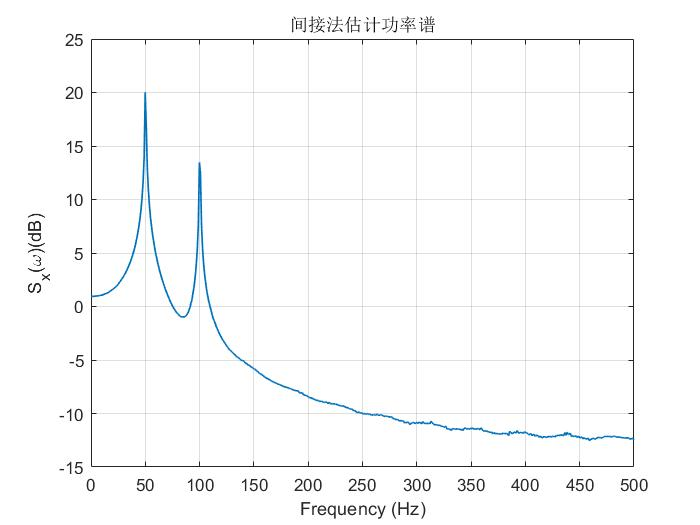
\includegraphics[width=10cm]{figs/f71.jpg}
    \caption{当$f_1=50Hz$,$f_2=100Hz$时的功率谱密度$S_x(\omega)$}
    \label{f71}
\end{figure}\newpage

2. 当$f_1=50Hz$,$ f_2=150Hz$,得到的结果如下图(\ref{f72})所示,
其中$S_x(\omega)$用$dB$表示。
\begin{figure}[htbp]
    \centering
    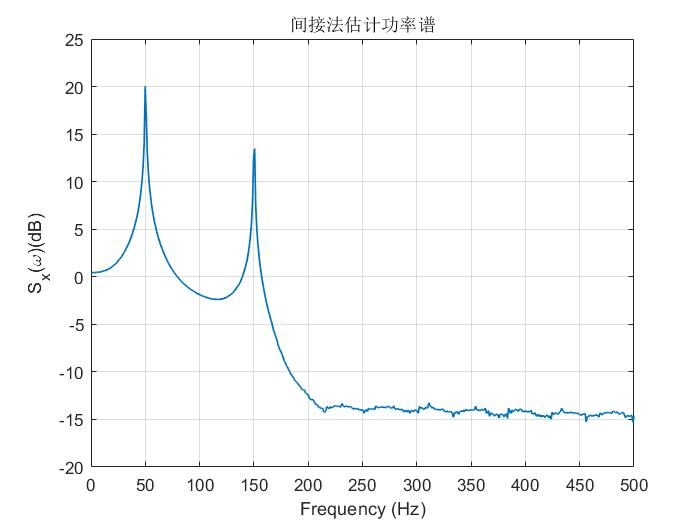
\includegraphics[width=10cm]{figs/f72.jpg}
    \caption{当$f_1=50Hz$,$f_2=150Hz$时的功率谱密度$S_x(\omega)$}
    \label{f72}
\end{figure}

3. 当$f_1=50Hz$,$ f_2=200Hz$,得到的结果如下图(\ref{f73})所示,
其中$S_x(\omega)$用$dB$表示。
\begin{figure}[htbp]
    \centering
    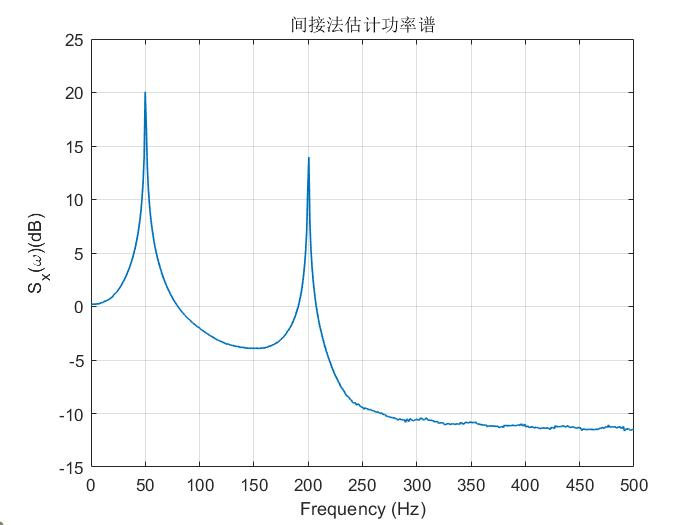
\includegraphics[width=10cm]{figs/f73.jpg}
    \caption{当$f_1=50Hz$,$f_2=200Hz$时的功率谱密度$S_x(\omega)$}
    \label{f73}
\end{figure}\newpage

4. 当$f_1=150Hz$,$ f_2=400Hz$,得到的结果如下图(\ref{f74})所示,
其中$S_x(\omega)$用$dB$表示。
\begin{figure}[htbp]
    \centering
    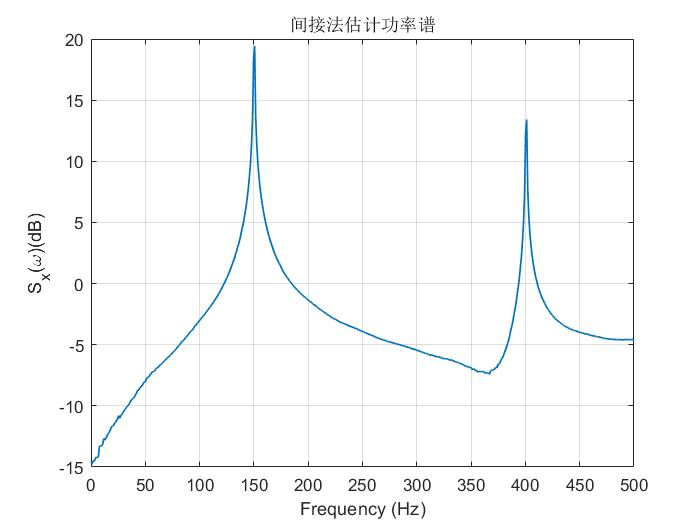
\includegraphics[width=10cm]{figs/f74.jpg}
    \caption{当$f_1=150Hz$,$f_2=400Hz$时的功率谱密度$S_x(\omega)$}
    \label{f74}
\end{figure}

5. 当$f_1=150Hz$,$ f_2=350Hz$,得到的结果如下图(\ref{f75})所示,
其中$S_x(\omega)$用$dB$表示。
\begin{figure}[htbp]
    \centering
    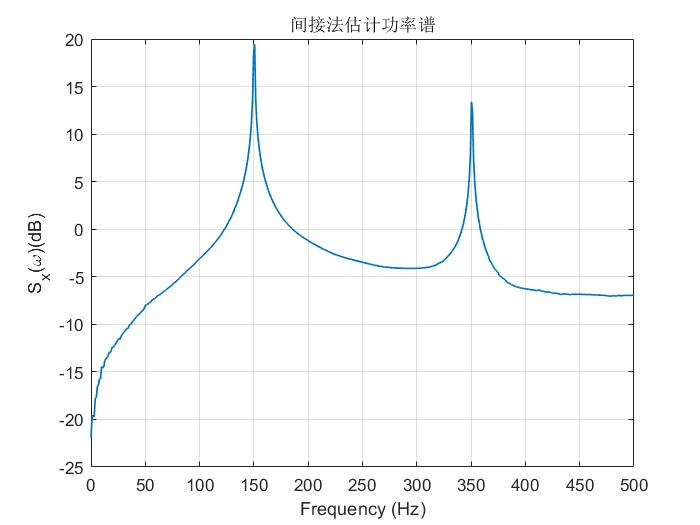
\includegraphics[width=10cm]{figs/f75.jpg}
    \caption{当$f_1=150Hz$,$f_2=350Hz$时的功率谱密度$S_x(\omega)$}
    \label{f75}
\end{figure}

\subsubsection{结果分析}
当改变正弦序列的频率组合,其功率谱密度上对应频率出现一个脉冲,
这与理论推到而来的公式是一致的。

\subsection{研究结论}
从节2.2.2所示的图谱中可以看出,直接法估计出的功率谱性能不好,其估计的分辨率很有限。
主要原因是直接法在估计时假定了数据窗以外的数据全为零,这样显然会有较大的误差。

从节2.3.2可看出用间接法所得功率谱估计图谱要相对平滑一些,
效果要较直接法为好。


\newpage 
\section{窄带随机过程题目一}
产生一高频窄带高斯序列,设计一系统以提取该序列的复振辐;
\subsection{研究过程}
1. 产生一个高斯窄带随机信号
\begin{lstlisting}[
	language = matlab, numbers=left, 
	numberstyle=\tiny,keywordstyle=\color{blue!70},
	commentstyle=\color{red!50!green!50!blue!50},frame=shadowbox,
	rulesepcolor=\color{red!20!green!20!blue!20},
	basicstyle=\ttfamily,
	]
%% 初始化设置
n=1:1000;
h=exp(-n);
%% 产生随机信号
c1=randn(1,1000);% 高斯白噪声序列
a=conv(c1,h);    
c2=randn(1,1000);
b=conv(c2,h);
fc=1e4;
x=zeros(1,1000);
for i=1:1000
    x(i)=a(i)*cos(2*pi*fc*i+2*pi*rand)
    -b(i)*sin(2*pi*fc*i+2*pi*rand);
end
\end{lstlisting}

2. 提取此信号的同向分量和正交分量,得到复包络为$\widetilde{A}(t)=a(t)+jb(t)$
\begin{lstlisting}[
	language = matlab, numbers=left, 
	numberstyle=\tiny,keywordstyle=\color{blue!70},
	commentstyle=\color{red!50!green!50!blue!50},frame=shadowbox,
	rulesepcolor=\color{red!20!green!20!blue!20},
	basicstyle=\ttfamily,
	]
for i=1:1000
aa(i)=a(i)+1i*b(i);
end
feather(aa);grid on;
title('复包络羽毛图');
\end{lstlisting}
\subsection{研究结果}
所得到的复包络的羽毛图如下图(\ref{f83})所示.
\begin{figure}[htbp]
    \centering
    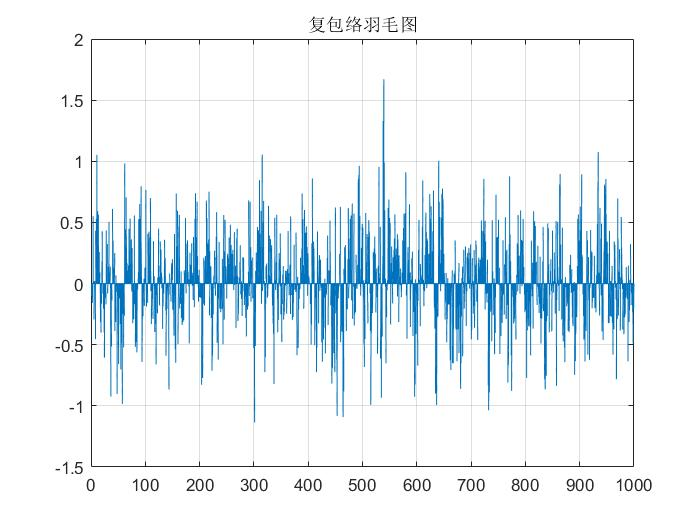
\includegraphics[width=10cm]{figs/f83.jpg}
    \caption{复包络羽毛图}
    \label{f83}
\end{figure}
\section{窄带随机过程题目二}
利用直方图研究序列的包络和相位的一维概率密度函数,并与理论结果进行比较。
\subsection{研究过程}
1. 求出包络(相位)的序列,并绘制其分布直方图。
\begin{lstlisting}[
	language = matlab, numbers=left, 
	numberstyle=\tiny,keywordstyle=\color{blue!70},
	commentstyle=\color{red!50!green!50!blue!50},frame=shadowbox,
	rulesepcolor=\color{red!20!green!20!blue!20},
	basicstyle=\ttfamily,
	]
for i=1:1000
    A(i)=(a(i)^2+b(i)^2)^(0.5);
end
histogram(A);grid on;
title('包络分布直方图');
\end{lstlisting}

2. 绘制出包络(相位)的一维概率密度函数
\begin{lstlisting}[
	language = matlab, numbers=left, 
	numberstyle=\tiny,keywordstyle=\color{blue!70},
	commentstyle=\color{red!50!green!50!blue!50},frame=shadowbox,
	rulesepcolor=\color{red!20!green!20!blue!20},
	basicstyle=\ttfamily,
	]
fa=ksdensity(A);
plot(fa,'linewidth',1);grid on;
title('一维概率密度');
\end{lstlisting}

3. 将分布直方图与一维概率密度函数进行对比
\subsection{研究结果}
包络的分布直方图如下图(\ref{f82})所示。
\begin{figure}[htbp]
    \centering
    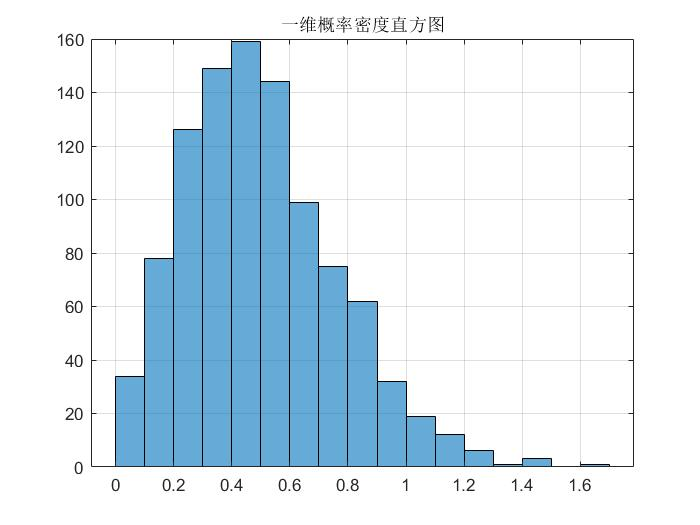
\includegraphics[width=10cm]{figs/f82.jpg}
    \caption{包络分布直方图}
    \label{f82}
\end{figure}

包络的一维概率密度如下图(\ref{f81})所示。
\begin{figure}[htbp]
    \centering
    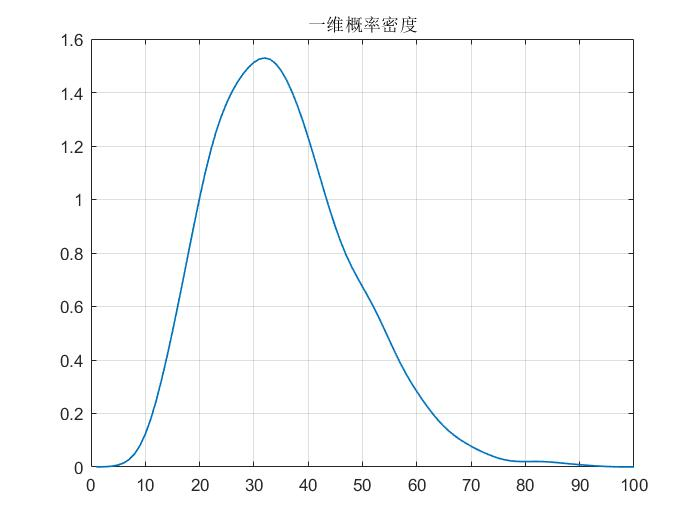
\includegraphics[width=10cm]{figs/f81.jpg}
    \caption{包络一维概率密度}
    \label{f81}
\end{figure}

相位的分布直方图如下图(\ref{f85})所示。
\begin{figure}[htbp]
    \centering
    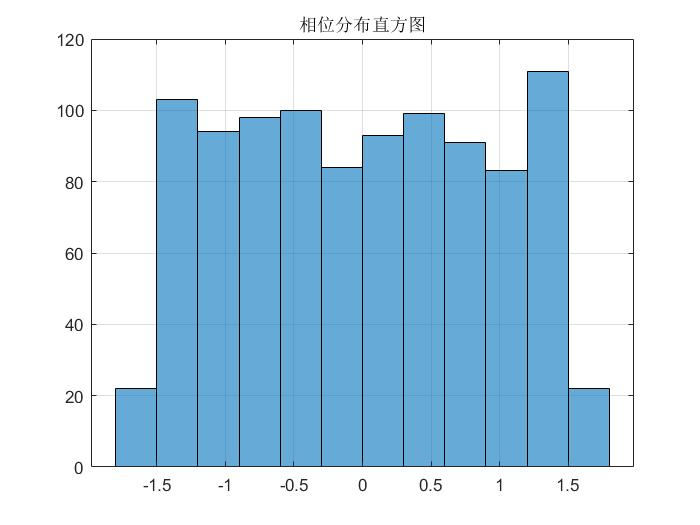
\includegraphics[width=10cm]{figs/f85.jpg}
    \caption{相位分布直方图}
    \label{f85}
\end{figure}
\newpage
相位的一维概率密度如下图(\ref{f84})所示。
\begin{figure}[htbp]
    \centering
    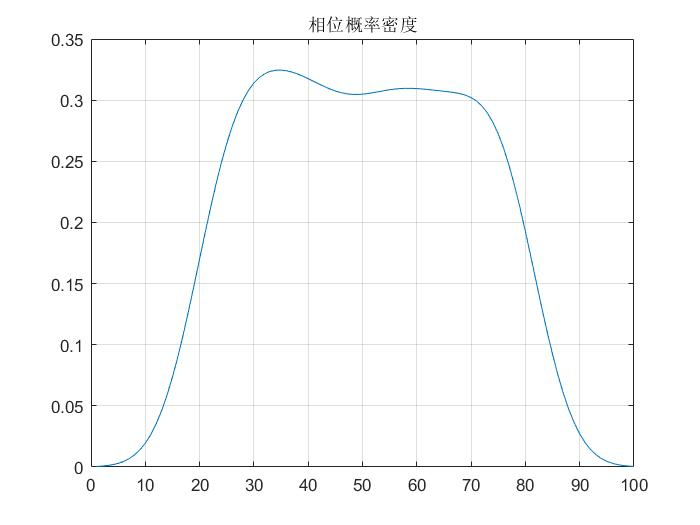
\includegraphics[width=10cm]{figs/f84.jpg}
    \caption{相位一维概率密度}
    \label{f84}
\end{figure}
\subsection{结果分析}

包络序列的分布直方图和相位序列的分布直方图均和理论值拟合较好。
\section{研究总结}

本次大作业中,加强了利用MATLAB对随机信号进行分析的能力,通过实践和仿真
,使抽象的理论知识可视化,巩固了理论知识,加深了对有关随机过程的知识的
理解,如功率谱密度的两种定义方法,信号起伏程度和带宽的关系,以及窄带
随机信号包络和相位的分布等。

另外,还训练了利用MATLAB进行滤波器设计的能力,利用MATLAB进行滤波器设计
有两种常用方法,一种是直接编写MATLAB代码产生滤波器,另一种是利用Filter
Designer APP设计滤波器,利用FD APP设计滤波器更为快速和简便,并可以直接生成
滤波器的MATLAB代码。
\end{document}